%
% name: final-pres.tex 
% tex file for design presentation 
%
% date last modified: 5 may 2018
% modified by: jerry 
%

\documentclass[xcolor=table]{beamer}
\hypersetup{pdfpagemode=FullScreen}
\mode<presentation> {
%\usetheme{default}
%\usetheme{AnnArbor}
%\usetheme{Antibes}
%\usetheme{Bergen}
%\usetheme{Berkeley}
%\usetheme{Berlin}
%\usetheme{Boadilla}
%\usetheme{CambridgeUS}
%\usetheme{Copenhagen}
%\usetheme{Darmstadt}
%\usetheme{Dresden}
%\usetheme{Frankfurt}
%\usetheme{Goettingen}
%\usetheme{Hannover}
%\usetheme{Ilmenau}
%\usetheme{JuanLesPins}
%\usetheme{Luebeck}
%\usetheme{Madrid}
%\usetheme{Malmoe}
%\usetheme{Marburg}
%\usetheme{Montpellier}
%\usetheme{PaloAlto}
%\usetheme{Pittsburgh}
\usetheme{Rochester}
%\usetheme{Singapore}
%\usetheme{Szeged}
%\usetheme{Warsaw}

% As well as themes, the Beamer class has a number of color themes
% for any slide theme. Uncomment each of these in turn to see how it
% changes the colors of your current slide theme.

%\usecolortheme{albatross}
%\usecolortheme{beaver}
%\usecolortheme{beetle}
\usecolortheme{crane}
%\usecolortheme{dolphin}
%\usecolortheme{dove}
%\usecolortheme{fly}
%\usecolortheme{lily}
%\usecolortheme{orchid}
%\usecolortheme{rose}
%\usecolortheme{seagull}
%\usecolortheme{seahorse}
%\usecolortheme{whale}
%\usecolortheme{wolverine}
\useinnertheme{rectangles}

%\setbeamertemplate{headline}{}
%\setbeamertemplate{footline} % To remove the footer line in all slides uncomment this line
%\setbeamertemplate{footline}[page number] % To replace the footer line in all slides with a simple slide count uncomment this line
\setbeamertemplate{navigation symbols}{} % To remove the navigation symbols from the bottom of all slides uncomment this line
}

% points to our sas image directory for loading diagrams
\graphicspath{{../../sas/images/}}

\usepackage{tikz}
\usepackage{tabularx}
\usepackage{amsmath}
\usepackage{caption}
\usepackage{centernot}
\usepackage{graphicx} % Allows including images
\usepackage[absolute,overlay]{textpos}
\usepackage{booktabs} % Allows the use of \toprule, \midrule and \bottomrule in tables

\newcommand\tab[1][1cm]{\hspace*{#1}}
\definecolor{bgcolor}{HTML}{ffcc66}

%----------------------------------------------------------------
%   TITLE PAGE
%----------------------------------------------------------------
\title{
\textbf{Final Presentation} \\ \small{Team 3: Download of public facing data for registered users}
} 

\author{
Jerry Bonnell
\and Gururaj Shriram
\and Lixiong Liang
\and Heyu Yao
\and Erica Chang 
} % Your name
\date{May 7, 2018} % Date, can be changed to a custom date

\begin{document}

%-----------------------------------------------------------------------
%   PRESENTATION SLIDES
%------------------------------------------------------------------------
\begin{frame}[plain]
	\titlepage
\end{frame}

\begin{frame}
	\frametitle{Agenda}
	\tableofcontents
\end{frame}

\section{Requirements}
\setbeamercolor{background canvas}{bg=bgcolor}
\begin{frame}[plain]
	\Huge{\centerline{Requirements}}
\end{frame}
\setbeamercolor{background canvas}{bg=white}

\begin{frame}
	\frametitle{Project Purpose}
	\begin{itemize}
		\item Users are interested in \textbf{downloading}:
		      \begin{block}{Data types}
			      \begin{enumerate}
					  \item \textbf{Cadastral} data - points and polygons on a map
					  % could be dimensions and area of a parcel of land
					  \item \textbf{``Storytelling''} data - images, videos, audio files, etc. % could be an interview recorded on a day
			      \end{enumerate}
			  \end{block}
        \vspace{4px}
		\item \textbf{Purpose:} Users can create their own maps from this data
			\begin{itemize}
				\item e.g. a map pertaining to bus stop information
				\item Expedites the process of receiving land titles.
			\end{itemize}
	\end{itemize}
\end{frame}

\begin{frame}
	\frametitle{Functional Requirements}
	% user must be able to download data in an output format they request. 
	% that data consists of storytelling/multimedia data as well as 
	% cadastral data 
	\begin{itemize}
		\item User can choose an \textbf{output format} for queried data and 
		download \textbf{locally} to computer. 
		\begin{itemize}
			\item \textbf{Cadastral} data: Convert data to \texttt{Geojson, 
			KML, shapefile, CSV}
			\begin{itemize}
				\item<2-> Also \texttt{topojson}! %geojson that encodes topology
			\end{itemize}
			\item \textbf{``Storytelling''} data: fetch directly for each 
			request
		\end{itemize}
	\end{itemize}
\end{frame}

\begin{frame}
	\frametitle{Non-functional Requirements}
	\begin{itemize}
		\item Must handle up to 3 \textbf{simultaneous} requests. \\ 
		\item <2-> \textcolor{purple}{\textit{Tried up to 100 
		simultaneous requests!}}
	\end{itemize}
\end{frame}

\section{Architecture}
\setbeamercolor{background canvas}{bg=bgcolor}
\begin{frame}[plain]
	\Huge{\centerline{Architecture}}
\end{frame}
%------------------------------------------------
\setbeamercolor{background canvas}{bg=white}
\begin{frame}
	\frametitle{Architectural Style: Three-tier}
	\begin{center}
		\bgroup
		\def\arraystretch{2}
		% generated table online, hence the mess 
		\begin{tabular}{|c|}
			\hline
			\rowcolor[HTML]{EF5350} 
			\multicolumn{1}{|c|}{\cellcolor[HTML]{EF5350}{\color[HTML]{FFFFFF} Client-server tier: Allows download server to handle requests}} \\ \hline
			\rowcolor[HTML]{E53935} 
			{\color[HTML]{FFFFFF} Business tier: converts and archives data} \\ \hline
			\rowcolor[HTML]{B71C1C} 
			{\color[HTML]{FFFFFF} Database-centric tier: requests geospatial data from database} \\ \hline
		\end{tabular}
		\egroup
	\end{center}
\end{frame}
%------------------------------------------------
\begin{frame}
	\frametitle{System Diagram}
		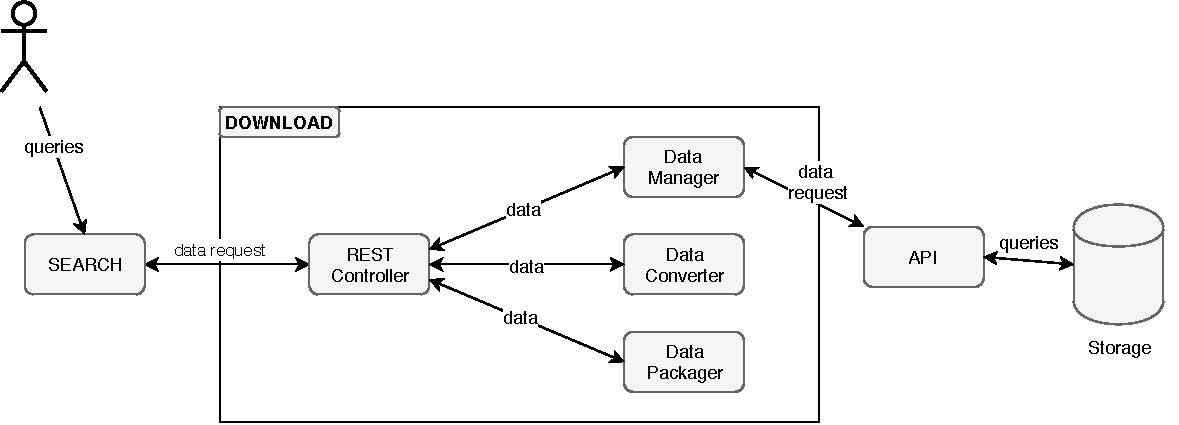
\includegraphics[width=\linewidth]{component.pdf}
\end{frame}
%------------------------------------------------
\begin{frame}
	\frametitle{Class Diagram}
	\begin{center}
		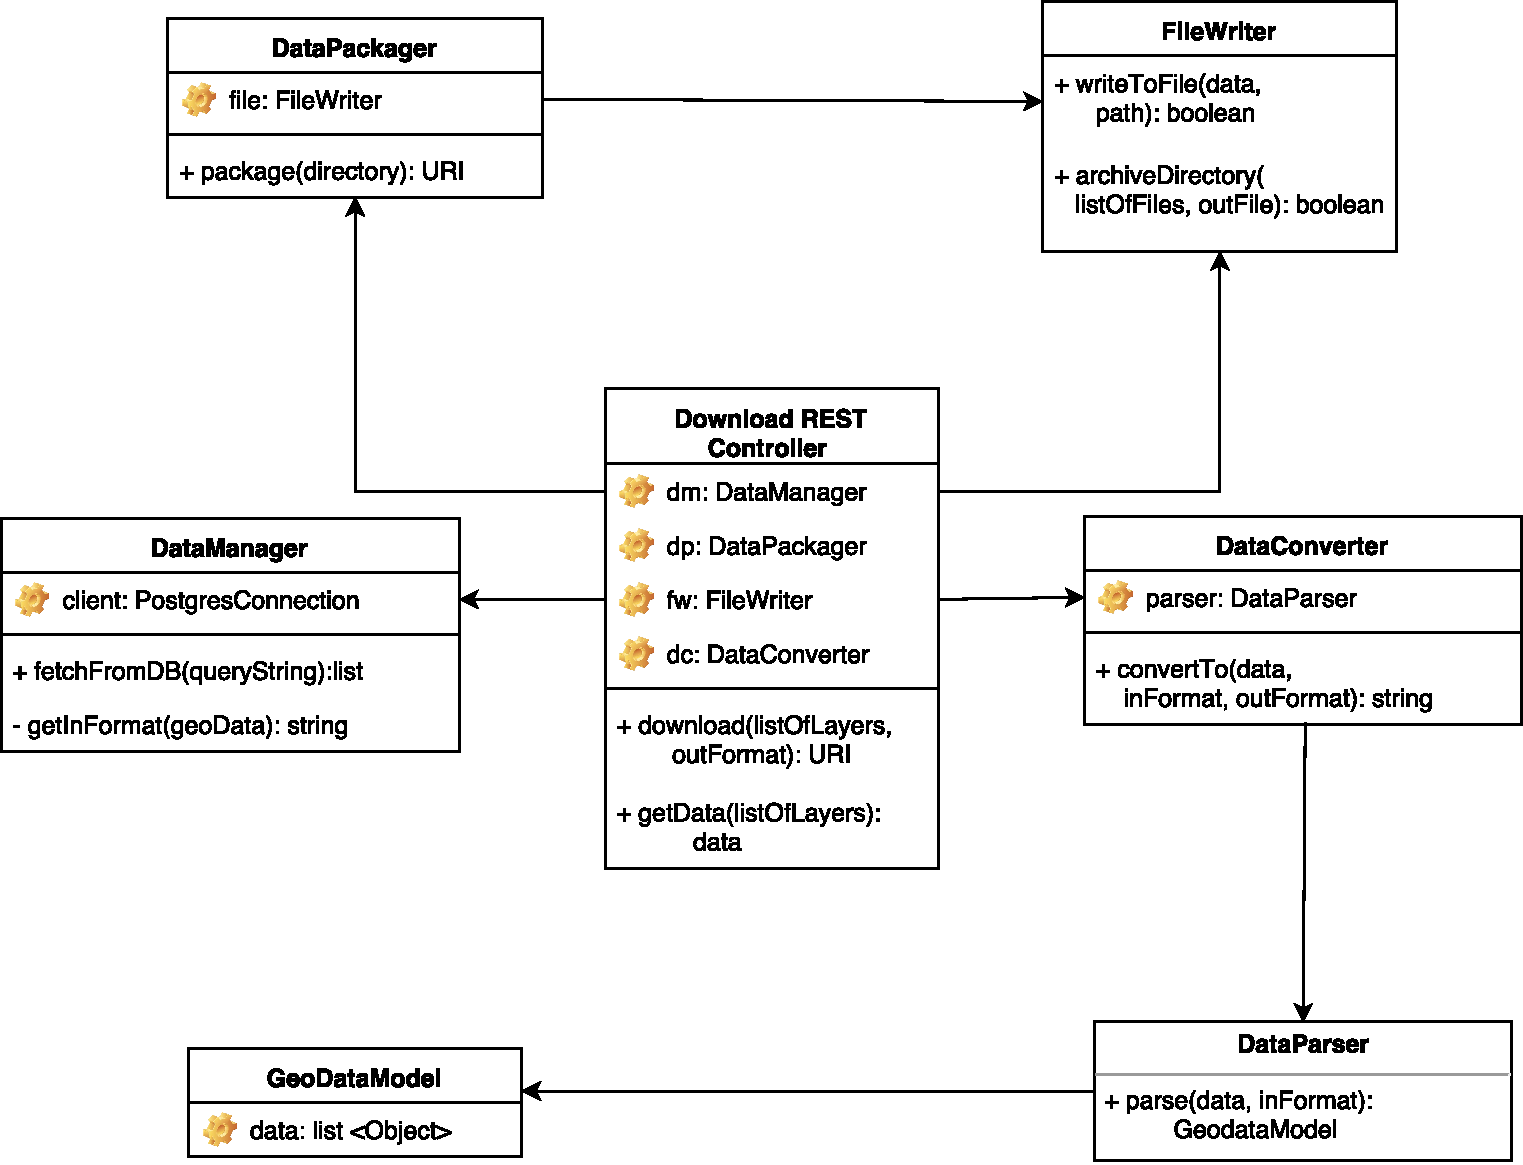
\includegraphics[width=0.8\linewidth]{class_diagram.pdf}
	\end{center}
\end{frame}
%-----------------------------------------------
\begin{frame}[plain]
	\frametitle{Sequence Diagram}
	\begin{center}
		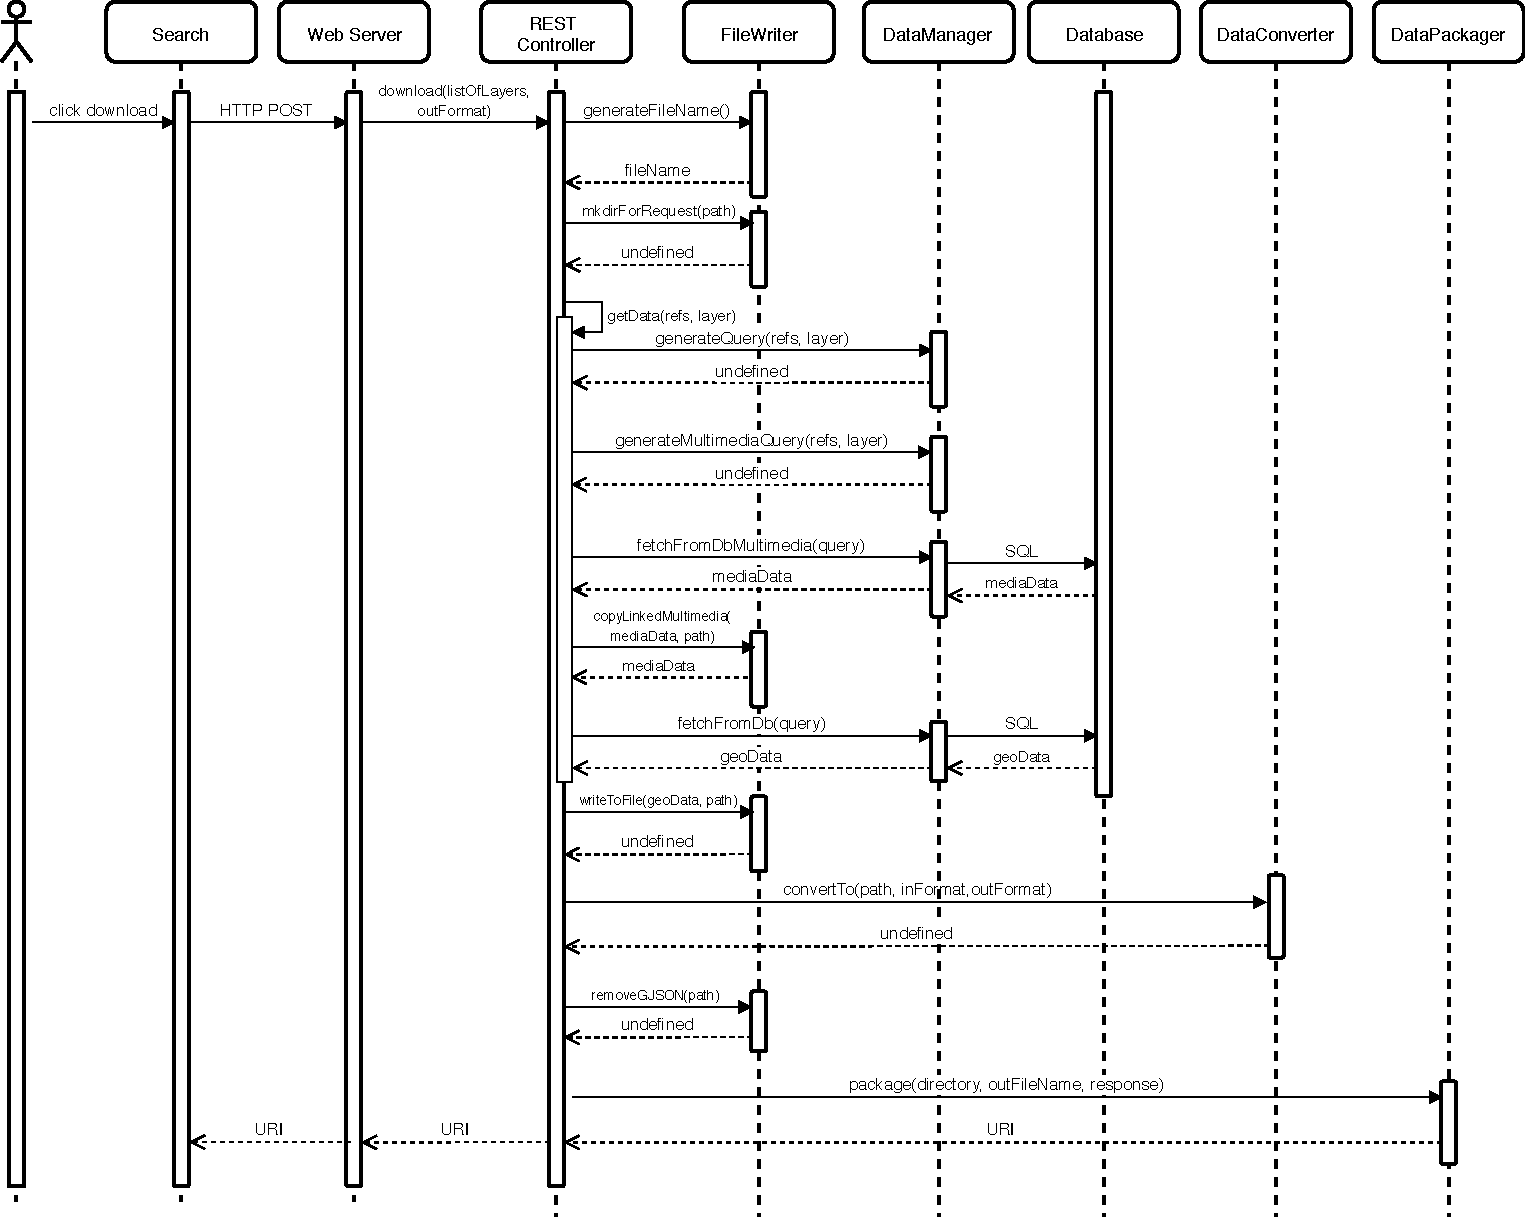
\includegraphics[width=0.9\linewidth]{sequence_diagram.pdf}
	\end{center}
\end{frame}
%=====================================================
\section{Demo!}
%-----------------------------------------------------
\setbeamercolor{background canvas}{bg=bgcolor}
\begin{frame}[plain]
	\Huge{\centerline{Demo!}}
\end{frame}
%----------------------------------------------------
\setbeamercolor{background canvas}{bg=white}
\begin{frame}[plain]
	\Huge{\centerline{Questions?}}
\end{frame}

\end{document}
